\subsection{Reading temperature}\label{subsec:reading-temperature}

The next requirement is reading the outside temperature.
This step is necessary to react to the environment and to stop or increase distribution of the formic acid.
As previously established, delivering formic acid below 10 °C must be stopped, as its melting point is already at 8.4 °C.
Furthermore, the following volume per hour of distribution depending on the temperature are established as part of this requirement.
The distribution is also stopped at temperature exceeding 30 °C, as measurement have shown that the humidity is usually too high to effectively evaporate formic acid.

\begin{table}[h]
    \centering
    \caption{Volume per hour depending on outside temperature}
    \label{tab:volume-per-hour-depending-on-temperature}
    \renewcommand{\arraystretch}{1.2}
    \begin{tabular}{l|l}
        Temperature range & Volume per hour [ml/h] \\
        \hline
        $\leq$ 10 °C & 0 \\
        $ > $ 10 °C $\leq$ 15 °C & 0.5 \\
        $ > $ 15 °C $\leq$ 20 °C & 1 \\
        $ > $ 20 °C $\leq$ 25 °C & 1.5 \\
        $ > $ 25 °C $\leq$ 30 °C & 1 \\
        $ > $ 30 °C & 0
    \end{tabular}
\end{table}

\newpage
\begin{lstlisting}[label={lst:react-to-temperature},language=C++, caption=Determining volume based on temperature]
float getPumpAmount(float temperature) {
    if (temperature <= 10.0f) {
        return 0.0f;
    } else if(temperature <= 15.0f) {
        return 0.5f;
    } else if(temperature <= 20.0f) {
        return 1.0f;
    } else if(temperature <= 25.0f) {
        return 1.5f;
    } else if(temperature <= 30.0f) {
        return 1.0f;
    }

    return 0.0f;
}

bool mustContinuePumping(float temperature) {
    return getPump()->pumpedMilliliter(millis()) < getPumpAmount(temperature);
}

void loop() {
     if (millis() - lastSensorReadingsTime >= ONE_HOUR) {
        SensorReadings sensorReadings = readHumidityAndTemperature();
        lastSensorReadings = sensorReadings;
        ...
    }
    ...
    if (millis() - lastPumpCycle >= ONE_HOUR) {
        ...
        getPump()->start(millis());

        while(mustContinuePumping(lastSensorReadings.temperature)) {
            delay(100);
        }
        ...
            getPump()->stop();
        ...
    }
}
\end{lstlisting}

In Listing \ref{lst:react-to-temperature}, the code to determining if the pump should be active or not is shown.
The function \textit{getPumpAmount} returns the amount to be pumped in milliliters, based on the input \textit{temperature}.
This value is used in \textit{mustContinuePumping} to return true, if the pump must still be pumping to reach that value, or false otherwise.

In the main loop of the program, first the temperature is read.
As previously described, this is done once every hour.
The pump is then started and the program is halted as long as \textit{mustContinuePumping} returns true.
Since the pump was started before, it is still running while the program is halted.
After the function returns false, the pump is stopped again.

\begin{figure}[h]
    \centering
    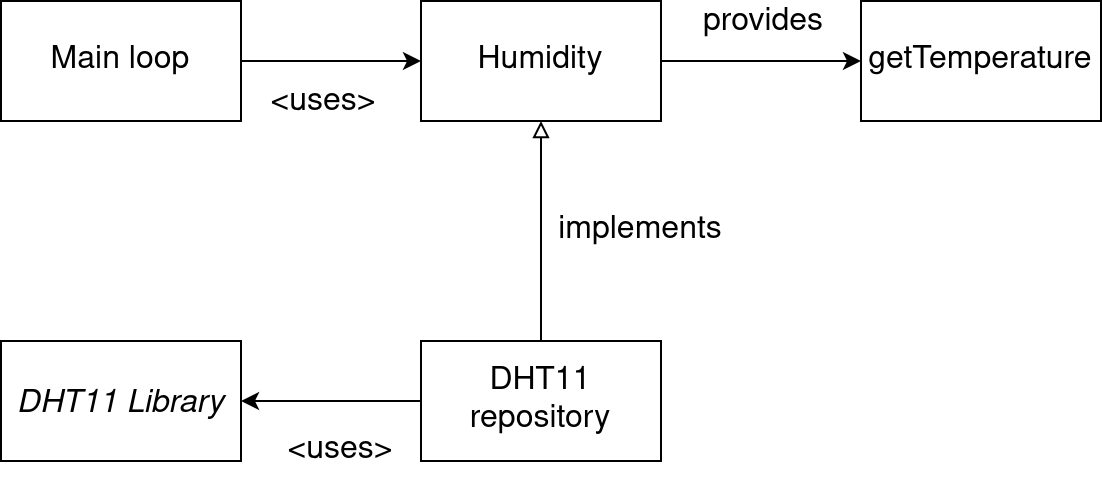
\includegraphics[width=0.5\textwidth]{img/humidity-architecture}
    \caption{Abstraction of the DHT11 library and its usage}
    \label{fig:abstraction-of-dht11}
\end{figure}

The temperature itself is read using a library made to interact with the DHT11 sensor.
This interaction is highly abstracted, which makes it unpractical to show the code itself.
In Figure \ref{fig:abstraction-of-dht11}, this abstraction is visualised.
The main loop only uses a high level abstraction, which provides a function to retrieve the temperature.
A class that interacts with the library, i.e., the sensor, implements this abstraction.
This architecture allows switching sensor types, if necessary, with only minimal code changes.
